%************************************************
\chapter{Q-learning with CVaR}\label{ch:qlearning}
%************************************************

While value iteration is a useful algorithm, it only works when we have complete knowledge of the environment - including the probability transitions $p(x'|x,a)$. This is often not the case in practice and we have to rely on different methods, based on direct interaction with the environment. One such algorithm is the well-known Q-learning which we explore in this chapter.

We first remind the reader of Q-learning basics in \secref{qlearning} and introduce CVaR estimation in \secref{cvarestimation}. These concepts are combined together with CVaR value iteration and in \secref{qcvar} we propose the first CVaR Q-learning algorithm. We treat the optimal policy separately in \secref{qpolicy}.

The algorithm is then experimentally verified on suitable environments in \secref{qexperiments}.

%***********************************************************************************************************************************************************
%***********************************************************************************************************************************************************
%***********************************************************************************************************************************************************
\section{Q-learning}\label{sec:qlearning}

Q-learning (\citet{watkins1992q}) is an important off-policy temporal difference control algorithm, that works by repeatedly updating the $Q$ value estimate according to the sampled rewards and states using a moving exponential average.
\begin{equation}
\begin{split}
&Q_{t+1}(x, a) = (1-\beta_t)Q_{t}(x, a) + \beta_t\bsquare{r + \gamma \max_{a'} Q_t(x', a')}\\
&x' \sim p(\cdot|x, a)
\end{split}
\end{equation}
Here $Q$ is an estimate of the optimal action-value function \eqnref{q} and $\beta_t$ is the learning rate at time $t$. The expression $r + \gamma \max_{a'} Q_t(x', a')$ is called a \textit{target} and is sometimes denoted as $\cT Q$. The idea of the algorithm is to bring the value function closer to the target, which is more 'informed' than the original value since it has information about the reward and next state, which came directly from the sampled transition. The optimal value of $Q(x, a)$ is then the expected target, which we reach in the limit.

The order of the visited states is unimportant, as long as all reachable states are updated infinitely often and the learning rate meets a standard condition used in stochastic approximation.
\begin{equation}\label{eqn:beta}
\sum_{t=0}^\infty \beta_t = \infty  \quad \sum_{t=0}^\infty \beta_t^2 < \infty\\
\end{equation}
See \citet{jaakkola1994convergence} for details.

While the algorithm would converge if we were using a completely random policy, in practice we often try to speed up the convergence by using a smarter, yet still random policy as seen in \algref{qlearning}.


\begin{algorithm}
\caption{Q-learning}
\begin{algorithmic}\label{alg:qlearning}
    \STATE Initialize $Q(x, a)$ for all $x \in \cX, a \in \cA$ arbitrarily, and $Q(x_\text{terminal}, \cdot) = 0$
    
	\FOR{each episode}
	
	\STATE $x = x_0$
	
	\WHILE{$x$ is not terminal}
	\STATE Choose $a$ using a policy derived from $Q$ (e.g. $\varepsilon$-greedy)
	\STATE Take action $a$, observe $r, x'$
	\STATE $Q(x, a) = (1-\beta_t)Q(x, a) + \beta_t\bsquare{r + \gamma \max_{a'} Q(x', a')}$
	\STATE $x = x'$	
	\ENDWHILE
	
	\ENDFOR
\end{algorithmic}
\end{algorithm}


\section{CVaR estimation}\label{sec:cvarestimation}

Before formulating a CVaR version of Q-learning, we must first talk about simply \emph{estimating} CVaR, as it is not as straightforward as the estimation of expected value.

Let us remind ourselves of the primal definition of CVaR \eqnref{cvarprimal}:
\begin{equation*}
\cvar_\alpha(Z)=
\max_s\left\lbrace \dfrac{1}{\alpha}\expect
\left[ (Z-s)^-\right] + s  \right\rbrace 
\end{equation*}
If we knew the exact $s^*=\var_\alpha$, we could estimate the CVaR as a simple expectation of the $\dfrac{1}{\alpha}(Z-s^*)^-+s^*$ function. As we do not know this value in advance, a common approach is to first approximate $\var_\alpha$ from data, then use this estimate to compute it's $\cvar_\alpha$. This is usually done with a full data vector, requiring the whole data history to be saved in memory.

When dealing with reinforcement learning, we would like to store our current estimate as a scalar instead. This requires finding a recursive expression whose expectation is the CVaR value. Fortunately, similar methods have been thoroughly investigated in the stochastic approximation literature by \citet{robbins1951stochastic}.

The RM theorem has also been applied directly to CVaR estimation by \citet{bardou2009recursive}, who used it to formulate a recursive importance sampling procedure useful for estimating CVaR of long-tailed distributions.

First let us describe the method for a one step estimation, meaning we sample values (or rewards in our case) $r$ from some distribution and our goal is to estimate CVaR at a given confidence level $\alpha$. The procedure requires us to maintain two separate estimates $V$ and $C$, being our VaR and CVaR estimates respectively.
\begin{align}
V_{t+1} &= V_{t} + \beta_t \bsquare{1-\dfrac{1}{\alpha}\indicator_{(V_t \ge r)}}\label{eqn:varestimate}\\
C_{t+1} &= (1-\beta_t)C_t + \beta_t \bsquare{V_t + \dfrac{1}{\alpha}(r-V_t)^-}\label{eqn:cvarestimate}
\end{align}
An observant reader may recognize a standard equation for quantile estimation in equation \eqnref{varestimate} (see e.g. \citet{koenker2001quantile} for more information on quantile estimation/regression). The expectation of the update $\expect\bsquare{1-\dfrac{1}{\alpha}\indicator_{(V_t \ge r)}}$ is the inverse gradient of the CVaR primal definition, so we are in fact performing a Stochastic Gradient Descent on the primal.

Equation \eqnref{cvarestimate} is also quite intuitive, representing the moving exponential average of the primal CVaR definition \eqnref{cvarprimal}. The estimations are proven to converge, given the usual requirements on the learning rate \eqnref{beta} \citep{bardou2009recursive}.

%***********************************************************************************************************************************************************
%***********************************************************************************************************************************************************
%***********************************************************************************************************************************************************

\section{CVaR Q-learning}\label{sec:qcvar}

We now extend the previously established CVaR Value Iteration and combine it with the recursive CVaR estimation techniques to formulate a new algorithm we call CVaR Q-learning.

\subsection{Temporal Difference update}
We first define two separate values for each state, action and atom $V, C: \cX\times\cA\times\cY\to\real$ where $C(x, a, y)$ represents $\cvar_y(Z(x, a))$ of the distribution, similar to the definition \eqnref{cdef}. $V(x, a, y)$ represents the $\var_y$ estimate, or the estimate of the $y-$quantile of a distribution recovered from $\cvar_y$ by Lemma \ref{thm:varcvarconnection}.

A key to any temporal difference algorithm is it's update rule. The CVaR TD update rule extends the improved value iteration procedure and we present the full rule for uniform atoms in \algref{cvartd}. 

Let us now go through the algorithm step by step. We first construct a new CVaR (line \ref{alg:cvartd:1}), representing $\cvar_y(Z(x'))$, by greedily selecting actions that yield the highest CVaR for each atom. This is in contrast with both standard Q-learning and Quantile Regression Q-learning (\secref{dqn:qrdqn}) where we select a single action for the whole distribution.
This step is implicit in the CVaR value iteration procedure since we are not working with action-value functions. 

The new values $C(x', \bigcdot)$ are then transformed to the underlying distribution (line \ref{alg:cvartd:2}) $\mathbf{d}$ and transformed to the target $\cT \mathbf{d} = r + \gamma \mathbf{d}$. A natural Monte Carlo approach would be then to generate samples from this target distribution and use these to update our estimates $V, C$.

Since we know the distribution estimates exactly, we do not have to actually sample - instead we use the quantile values proportionally to their probabilities (in the uniform case, this means exactly once) and apply the respective VaR and CVaR update rules (lines \ref{alg:cvartd:4}, \ref{alg:cvartd:5}).


\begin{algorithm}
\caption{CVaR TD update - uniform case}
\begin{algorithmic}[1]\label{alg:cvartd}

    \STATE \textbf{input:} $x, a, x', r$
    
    \FOR{each $i$ }
	\STATE $C(x', y_i) = \max_{a'} C(x', a', y_i)$ \label{alg:cvartd:1}
	\ENDFOR
	
	\STATE $\mathbf{d}= \text{extractDistribution}\bround{C(x', \bigcdot), \mathbf{y}}$ \comment{See \algref{cvarvi}}\label{alg:cvartd:2}

	\FOR{each $i, j$}
	\STATE $V(x, a, y_i) = V(x, a, y_i) + \beta \bsquare{1 - \frac{1}{y_i}\indicator_{(V(x, a, y_i) \ge r+\gamma d_j)}}$  \label{alg:cvartd:4}
	\STATE $C(x, a, y_i) = (1-\beta)C(x, a, y_i) + \beta\bsquare{V(x, a, y_i) + \frac{1}{y_i}\bround{r+\gamma d_j - V(x, a, y_i)}^-}$\label{alg:cvartd:5}
	\ENDFOR
\end{algorithmic}
\end{algorithm}

If the atoms aren't uniform, we have to perform basic importance sampling when updating the estimates. See \algref{cvartdg} for a general version of the TD update. In contrast with the uniform version, we iterate only over the atoms and perform a single update for the whole target by taking an expectation over the target distribution. 

This is a valid approach since the sample mean is equal to the mean of the original distribution. In this case we are performing the updates on batches of samples and the final expected value remains unchanged.
\begin{equation*}
\mathbb{E}[f(Z)] = \sum_i p_i \mathbb{E}[f(Z_i)]
\end{equation*}
The above equation holds for any function $f$ if $Z$ is a mixture of $Z_i$, so it also holds for the VaR update $1 - \frac{1}{y_i}\indicator_{(V(x, a, y_i) \ge r+\gamma d_j)}$ where the learned distribution is a mixture of the different target distributions.

We conclude the same for the CVaR update, since the expectation remains unchanged. 

We are in fact using more informed updates - similar to the difference between pure and batch Stochastic Gradient Descent.

\begin{algorithm}
\caption{CVaR TD update - general case}
\begin{algorithmic}\label{alg:cvartdg}

    \STATE \textbf{input:} $x, a, x', r$
    
    \FOR{each $y_i$ }
	\STATE $C(x', y_i) = \max_{a'} C(x', a', y_i)$ \label{alg:cvartdg:1}
	\ENDFOR
	
	\STATE $\mathbf{d}= \text{extractDistribution}\bround{C(x', \bigcdot), \mathbf{y}}$ \label{alg:cvartdg:2} \comment{See \algref{cvarvi}}\label{alg:cvartd:2}

	\FOR{each $i$}
	\STATE $V(x, a, y_i) = V(x, a, y_i) + \beta \expect_j\bsquare{1 - \frac{1}{y_i}\indicator_{(V(x, a, y_i) \ge r+\gamma d_j)}}$  \label{alg:cvartd:4}
	\STATE $C(x, a, y_i) = (1-\beta)C(x, a, y_i) + \beta\expect_j\bsquare{V(x, a, y_i) + \frac{1}{y_i}\bround{r+\gamma d_j - V(x, a, y_i)}^-}$\label{alg:cvartdg:5}
	\ENDFOR
\end{algorithmic}
\end{algorithm}

\subsection{Note on convergence}
We do not prove the convergence of the CVaR Q-learning algorithm in this thesis as it would require significant work regarding convergence of the recursive CVaR estimation procedures. The update rules (\ref{eqn:varestimate}, \ref{eqn:cvarestimate})  have been only shown to converge if the underlying distributions are continuous \citep{bardou2009recursive}, which is not the case in our setting.


In the last section of this chapter, we show at least empirical convergence of the CVaR Q-learning algorithm.

%***********************************************************************************************************************************************************
%***********************************************************************************************************************************************************
%***********************************************************************************************************************************************************


\section{Optimal Policy}\label{sec:qpolicy}

Recall that in CVaR Value Iteration we can extract the optimal policy by recursively setting $y_{t+1}=y_t \xi^*_{x_{t+1}}$. This process is not straightforwardly extendable to our sample-based version of CVaR Value Iteration, since we would have to have acces to all possible transition states and probabilities in order to compute $\xi^*$.

Instead, we turn to the primal formulation of CVaR in what we call VaR-based policy improvement algorithm. We first introduce the VaR-based policy improvement in the context of distributional RL and prove it's validity. The policy improvement procedure is then used as a consistent heuristic for extracting the optimal policy from converged CVaR Value Iteration.


\subsection{VaR-based Policy Improvement}

Let us now assume that we have succesfully converged with distributional value iteration and have available the return distributions of some stacionary policy for each state and action. Our next goal is to find a policy improvement algorithm that will monotonically increase the $\cvar_\alpha$ criterion for selected $\alpha$.

Recall the primal definition of CVaR \eqnref{cvarprimal}
\begin{equation*}
\text{CVaR}_\alpha(Z)=
\max_s\left\lbrace \dfrac{1}{\alpha}\expect
\left[ (Z-s)^-\right] + s  \right\rbrace 
\end{equation*}
Our goal \eqnref{problem} can then be rewritten as
\begin{equation*}
\max_\pi CVaR_\alpha(Z^\pi) = \max_\pi \max_s \dfrac{1}{\alpha}\mathbb{E}
\left[ (Z^\pi-s)^-\right] + s
\end{equation*}
As mentioned earlier, the primal solution is equivalent to $\var_\alpha(Z)$
\begin{equation*}
\text{CVaR}_\alpha(Z)=
\max_s\left\lbrace \dfrac{1}{\alpha}\mathbb{E}
\left[ (Z-s)^-\right] + s  \right\rbrace =\dfrac{1}{\alpha}\mathbb{E}
\left[ (Z - \text{VaR}_\alpha(Z))^-\right] + \text{VaR}_\alpha(Z) 
\end{equation*}

The main idea of VaR-based policy improvement is the following: If we knew the value $s^*$ in advance, we could simplify the problem to maximize only
\begin{equation}\label{eqn:varbasedgoal}
\max_\pi CVaR_\alpha(Z^\pi) = \max_\pi \dfrac{1}{\alpha}\mathbb{E}
\left[ (Z^\pi-s^*)^-\right] + s^*
\end{equation}
Given that we have access to the return distributions, we can improve the policy by simply choosing an action that maximizes $\cvar_\alpha$ in the first state $a_0 = \text{arg}\max_\pi\text{CVaR}_\alpha(Z^\pi(x_0))$, setting $s^* = VaR_\alpha(Z(x_0))$ and focus on maximization of the simpler criterion.

This can be seen as coordinate ascent with the following phases:
\begin{enumerate}
\item Maximize $\frac{1}{\alpha}\mathbb{E}\left[ (Z^\pi(x_0)-s)^-\right] + s$ w.r.t. $s$ while keeping $\pi$ fixed. This is equivalent to computing CVaR according to the primal.
\item Maximize $\frac{1}{\alpha}\mathbb{E}\left[ (Z^\pi(x_0)-s)^-\right] + s$ w.r.t. $\pi$ while keeping $s$ fixed. This is the policy improvement step.
\item Recompute $\cvar_\alpha (Z^{\pi^*})$ where $\pi^*$ is the new policy.
\end{enumerate}
Since our goal is to optimize the criterion of the distribution starting at $x_0$, we need to change the value $s$ while traversing the MDP (where we have only access to $Z(x_t)$). We do this by recursively updating the $s$ we maximize by setting $s_{t+1} = \dfrac{s_t - r}{\gamma}$. See \algref{varbasedpi} for the full algorithm which we justify in the following theorem.

\begin{algorithm}
\caption{VaR-based policy improvement}
\label{alg:varbasedpi}
\begin{algorithmic}
    \STATE $a = \text{arg}\max_a \cvar_\alpha(Z(x_0, a))$
    \STATE $s = \var_\alpha(Z(x_0, a))$
    \STATE Take action $a$, observe $x, r$
    \WHILE{$x$ is not terminal}
    	\STATE $s = \dfrac{s-r}{\gamma}$
    	\STATE $a = \text{arg}\max_a \mathbb{E}\left[(Z(x, a)-s)^- \right]$
    	\STATE Take action $a$, observe $x, r$
   	\ENDWHILE
\end{algorithmic}
\end{algorithm}

\begin{theorem}
Let $\pi$ be a stationary policy, $\alpha \in (0, 1]$. 
By following policy $\pi'$ from algorithm \ref{alg:varbasedpi}, we improve $CVaR_\alpha(Z)$ in expectation:
$$CVaR_\alpha(Z^\pi) \le CVaR_\alpha(Z^{\pi'})$$ \todo{*'}
%
%Let policy $\pi'$ constructed the following way: Set $\pi'(x_0) = \text{arg}\max_\pi\cvar_\alpha(Z^\pi(x_0))$ and $s = \var_\alpha(Z^\pi(x_0, \pi'(x_0)))$. Each following step set $s = $
%

\end{theorem}

\begin{proof}

Let $s^*$ be a solution to $\frac{1}{\alpha}\mathbb{E}\left[ (Z^\pi(x_0)-s)^-\right] + s$. Then by optimizing $\max_\pi \dfrac{1}{\alpha}\mathbb{E}
\left[ (Z^\pi-s^*)^-\right]$, we monotonely improve the optimization criterion $CVaR_\alpha(Z(x_0))$.
\begin{align*}
\cvar_\alpha(Z^{\pi}) &= \max_{s}\dfrac{1}{\alpha}\mathbb{E}\left[ (Z^{\pi}-s)^-\right] + s &&= \dfrac{1}{\alpha}\mathbb{E}\left[ (Z^{\pi}-s^*)^-\right] + s^* \\
&\le \max_{\pi'}\dfrac{1}{\alpha}\mathbb{E} \left[ (Z^{\pi'}-s^*)^-\right] + s^* &&= \dfrac{1}{\alpha}\mathbb{E}\left[ (Z^{\pi^*}-s^*)^-\right] + s^*\\
 &\le \max_{s'}\dfrac{1}{\alpha}\mathbb{E}\left[ (Z^{\pi^*}-s')^-\right] + s' &&= CVaR_\alpha(Z^{\pi^*})
\end{align*}

When optimizing w.r.t. $\pi$ we can ignore the scaling term $\frac{1}{\alpha}$ and a constant term $s^*$ without affecting the optimal argument. We can therefore focus on optimization of $\mathbb{E}\left[ (Z^\pi(x_0)-s^*)^-\right]$.
\begin{equation}
\begin{split}
\mathbb{E}\left[(Z_t-s)^-\right] &= \mathbb{E}\left[(Z_t-s)\mathbb{1}(Z_t\le s)\right] = \mathbb{E}\left[(r_t + \gamma Z_{t+1}-s)\mathbb{1}(Z_{t+1}\le \dfrac{s - r_t}{\gamma})\right]\\
&= \sum_{x_{t+1}, r_t} P(x_{t+1}, r_t \given x_t, a)\mathbb{E}\left[(r_t + \gamma Z(x_{t+1})-s)\mathbb{1}(Z(x_{t+1})\le \dfrac{s - r_t}{\gamma})\right]\\
&= \sum_{x_{t+1}, r_t} P(x_{t+1}, r_t \given x_t, a)\mathbb{E}\left[\gamma\left(Z(x_{t+1})-\dfrac{s-r_t}{\gamma}\right)\mathbb{1}(Z(x_{t+1})\le \dfrac{s - r_t}{\gamma})\right]\\
&= \gamma\sum_{x_{t+1}, r_t} P(x_{t+1}, r_t \given x_t, a)\mathbb{E}\left[\left(Z(x_{t+1})-\dfrac{s-r_t}{\gamma}\right)\mathbb{1}(Z(x_{t+1})\le \dfrac{s - r_t}{\gamma})\right]\\
&= \gamma\sum_{x_{t+1}, r_t} P(x_{t+1}, r_t \given x_t, a)\mathbb{E}\left[\left(Z(x_{t+1}) - \dfrac{s - r_t}{\gamma}\right)^-\right]
\end{split}
\end{equation}
where we used the definition of return $Z_t = R_t + \gamma Z_{t+1}$ and the fact that probability mixture expectations can be computed as $\mathbb{E}[f(Z)] = \sum_i p_i \mathbb{E}[f(Z_i)]$ for any function $f$.

Now let's say we sampled reward $r_t$ and state $x_{t+1}$, we are still trying to find a policy $\pi^*$ that maximizes 
\begin{equation}\label{eqn:sampled x_t+1}
\begin{split}
\pi^* &=\text{arg}\max_\pi \mathbb{E}\left[(Z(x_t)-s)^-\right | x_{t+1}, r_t]\\
&= \text{arg}\max_\pi \mathbb{E}\left[\left(Z(x_{t+1}) - \dfrac{s - r_t}{\gamma}\right)^-\right]
\end{split}
\end{equation}

Where we ignored the unsampled states, since these are not a function of $x_{t+1}$, and the multiplicative constant $\gamma$ that will not affect the maximum argument.

At the starting state, we set $s=s^*$. At each following state we select an action according to equation \eqnref{sampled x_t+1}. By induction we maximize the criterion \eqnref{varbasedgoal} in each step.
\end{proof}

Note that while the resulting policy is nonstationary, we do not need an extended state-space to follow this policy. It is only necessary to remember our previous value of $s$.

The ideas presented here were partially explored by \citet{bauerle2011markov} although not to this extent. See Remark 3.9 in \citep{bauerle2011markov} for details.

\subsection{CVaR Q-learning extension}
We would now like to use the policy improvement algorithm in order to extract the optimal policy from CVaR Q-learning. This would mean optimizing $\mathbb{E}\left[(Z_t-s)^-\right]$ in each step. A problem we encounter here is that we have access only to the discretized distributions and we cannot extract the values between selected atoms.

As a solution to this, we propose an approximate heuristic that uses linear interpolation to extract the $\var$ of given distribution. 

The expression $\mathbb{E}\left[(Z_t-s)^-\right]$ is computed by taking the expectation of the distribution \textit{before} the value $s$. We are therefore looking for value $y$ where $\var_y=s$. This value is linearly interpolated from $\var_{y_{i-1}}$ and $\var_{y_{i}}$ where $y_i=\min \braces{y: \var_y \ge s}$. The expectation is then taken over the extracted distribution, as this is the distribution that approximates $\cvar$ the best.

See \algref{varbasedpolicy} for the exact procedure and \figref{linearinterp} for more intuition behind the heuristic.



\begin{algorithm}
\caption{CVaR Q-learning policy}\label{alg:varbasedpolicy}
\begin{algorithmic}
    \STATE \textbf{input:} $\alpha$, converged $V, C$
    		
	\STATE $x = x_0$
	\STATE $a = \argmax_a C(x, a, \alpha)$
	\STATE $s = V(x, a, y)$
	\WHILE{$x$ is not terminal}
	\STATE $\mathbf{d}_a = \text{extractDistribution}\bround{C(x', a, \bigcdot), \mathbf{y}}$ for each $a$
	\STATE $a = \argmax_a \text{expMinInterp}(s, \mathbf{d}, V(x', a, \bigcdot), \mathbf{y})$
	\STATE Take action $a$, observe $r, x'$
	\STATE $s = \dfrac{s-r}{\gamma}$
	\STATE $x = x'$
	\ENDWHILE

\hrulefill

	\STATE \comment{Compute $\mathbb{E}\left[(\mathbf{d}_a-s)^-\right]$ with linear interpolation}
	\STATE \textbf{function} expMinInterp  
\bindent
    \STATE \textbf{input:} $s$, vectors $\mathbf{d}, \mathbf{V}, \mathbf{y}$
    \STATE $z = 0$
    \FOR{$i \in \braces{1, ..., |\mathbf{y}|}$}
    	\IF{$S < V_i$}
		\STATE \textbf{break}
		\ENDIF
		\STATE $z = z + d_i\cdot(y_i - y_{i-1})$
	\ENDFOR
	
	\STATE $p_{\text{last}} = \dfrac{s - V_{i-1}}{V_{i}-V_{i-1}}(y_i - y_{i-1})$
	\STATE $z = z + d_i \cdot p_{\text{last}}$
	
	\STATE \textbf{output} $z$
\eindent
\end{algorithmic}
\end{algorithm}


%To side-step this issue, we bring the VaR-based improvement closer to CVaR Value Iteration and use it only in a one-step context. In each step, we compute the next $y$ as $F_{Z(x)}(\dfrac{s-r}{\gamma})$, which we extract from our VaR estimate $V$. Since we don't have access to the exact VaR for each $y \in [0,1]$ due to discretization, we use linear interpolaton as a heuristic. See \algref{varxibasedpolicy} for the full procedure.

%\begin{algorithm}
%\caption{CVaR Q-learning policy}\label{alg:varxibasedpolicy}
%\begin{algorithmic}
%    \STATE \textbf{input:} $\alpha$, converged $V, C$
%    		
%	\STATE $x = x_0$
%	\STATE $y = \alpha$
%	\WHILE{$x$ is not terminal}
%	\STATE $a = \argmax_a C(x, a, y)$
%	\STATE $s = V(x, a, y)$
%	\STATE Take action $a$, observe $r, x'$
%	\STATE $y = F_{Z(x')}(\dfrac{s-r}{\gamma})$
%	\STATE $x = x'$
%	\ENDWHILE
%\end{algorithmic}
%\end{algorithm}


%\begin{algorithm}
%\caption{Full CVaR Q-learning}
%\begin{algorithmic}
%    \STATE Initialize $V(x, a, y), C(x, a, y)$ for all $x\in\cX, a\in\cA, y\in\cY$ arbitrarily, and $C(x_\text{terminal}, \cdot, \cdot) = 0$
%    
%	\FOR{each episode}
%		
%	\STATE $x = x_0$
%	\STATE $y = \alpha$
%	\STATE $s = V(x, a, y)$
%	\WHILE{$x$ is not terminal}
%	\STATE Choose $a$ using a policy derived from $C, y$ (e.g. $\varepsilon$-greedy)
%	\STATE Take action $a$, observe $r, x'$
%	\STATE Update current estimates $V(x, a, y_i), C(x, a, y_i)$ (\algref{cvartd})
%	\STATE $y = F_{Z(x')}(\dfrac{s-r}{\gamma})$
%	\STATE $s = V(x, a, y)$
%	\STATE $x = x'$
%	\ENDWHILE
%	
%	\ENDFOR
%\end{algorithmic}
%\end{algorithm}


%*****************************************
%*****************************************
%*****************************************
\newpage

\section{Experiments}\label{sec:qexperiments}
We use the same gridworld from \secref{vi:experiments} with $\delta=0.1$. Since the positive reward is very sparse, we chose to run CVaR Q-learning on a smaller environment of size $10\times15$. We trained the agent for 10,000 sampled episodes with learning rate $\beta=0.4$ that dropped each 10 episodes by a factor of 0.995. The used policy was $\varepsilon-$greedy and maximized expected value ($\alpha=1$) with $\varepsilon=0.5$. Notice the high value of $\epsilon$. We found that lower $\epsilon$ values led to overfitting the optimal expected value policy as the agent updated states out of the optimal path sparsly. This point will be elaborated further in the experimental section of the next chapter.

With said parameters, the agent was able to learn the optimal policies for different levels of $\alpha$. See \figref{qgrid} for learned policies and \figref{qhist} for Monte Carlo comparisons.

\begin{figure}[h]
\center
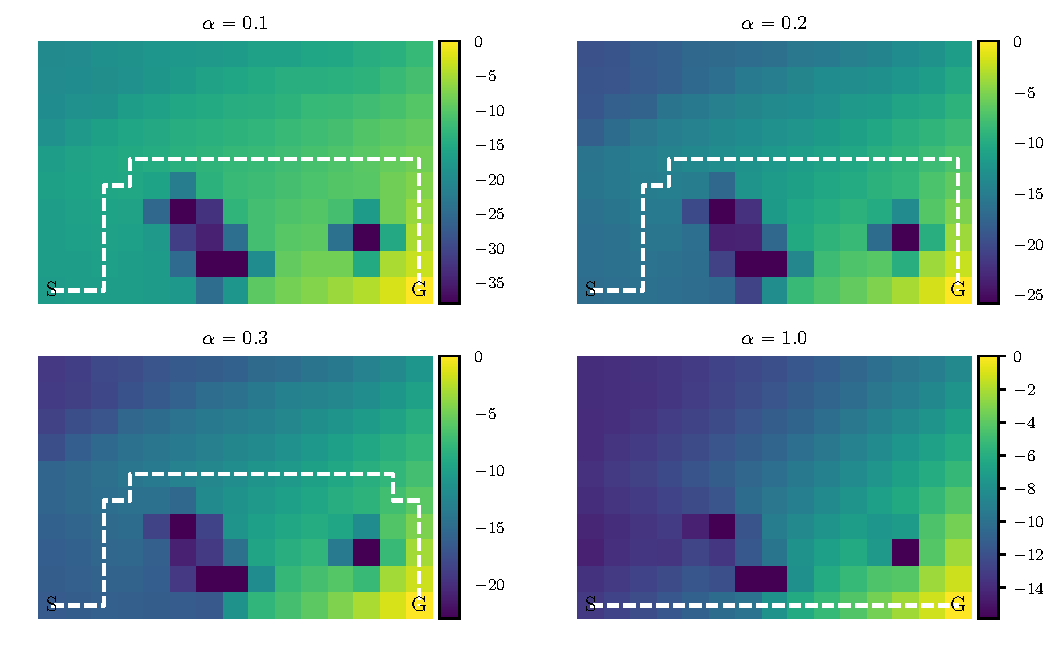
\includegraphics[width=\linewidth]{gfx/q_optimal_paths.pdf}
\caption{Grid-world Q-learning simulations. The optimal deterministic paths are shown together with CVaR estimates for given $\alpha$.}
\label{fig:qgrid}
\end{figure}


\begin{figure}[h]
\center
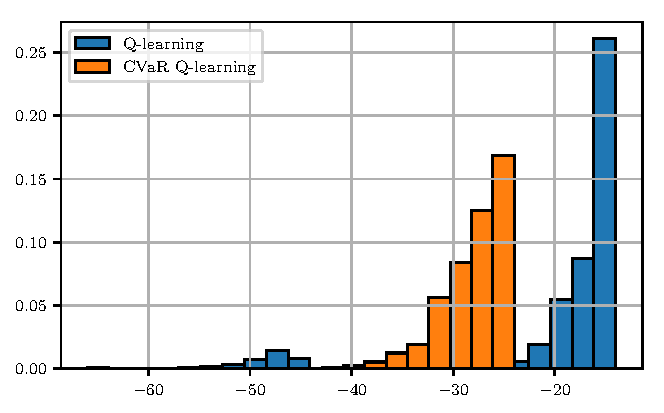
\includegraphics[width=0.6\linewidth]{gfx/sample_hist.pdf}
\caption{Histograms from 10000 runs generated by Q-learning and CVaR Q-learning with $\alpha=0.1$.}
\label{fig:qhist}
\end{figure}

The training was done with $N=50$ linearly-spaced atoms. We experimented with several discretization settings and didn't find many differences between log- and linearly-spaced points. Note that learning $\var$ and $\cvar$ for very low $\alpha$ values requires large number of samples and we found that extremely small atom values converged slowly.
\\
\\
\textit{Note on convexity:} Unlike CVaR Value Iteration, where we maintain convexity of the $y\cvar_y$ function with each update (given we started with convex estimates), in CVaR Q-learning we can break the convexity in each update for any atom. We experience this in practice as well as can be gauged from \figref{nonconvex}. Fortnately this fact does not break the update rule, since the targets we use to update $C$ as well as $V$ do not have to be in order.


\begin{figure}[h]
\center
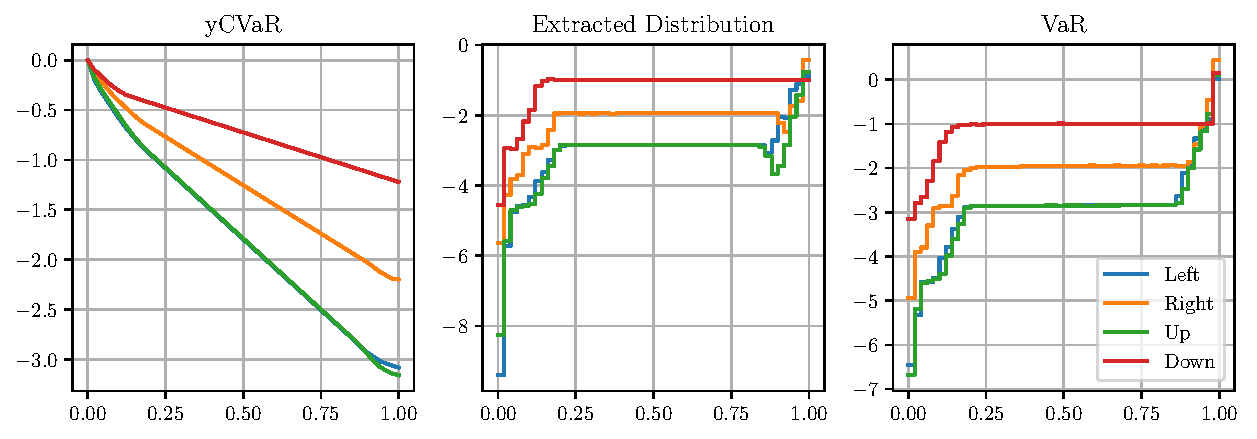
\includegraphics[width=\linewidth]{gfx/nonconvex.pdf}
\caption{Learned $C, V$ estimates for a single state after 10000 episodes. Notice the nonconvexities visible from the extracted distribution plot. Both extracted distribution and VaR functions should be nondecreasing.}
\label{fig:nonconvex}
\end{figure}

\unclear{Summary? just write more about the experiments, maybe multiple plots in appendix}



%*****************************************
%*****************************************
%*****************************************
%*****************************************
%*****************************************
